\section{Motivation}

Lebensmittelsicherheit ist strategisch für die Volksgesundheit und das Wohlbefinden der Gesellschaft. Der öffentliche Druck auf Hersteller für eine ausreichende Kennzeichnung von Produkten und ihre Bestandteile wird stetig größer.\\

Vom Rohstofflieferanten bis zum Endkunden gibt es ein Netz von Marktteilnehmern, die nur locker gekoppelt sind. Es gibt de facto kein Standard Informationsaustausch Verfahren. In der Fleischwarenindustrie zum Beispiel existieren weit über 140 unterschiedliche Austauschformate zwischen den Teilnehmern der Lieferkette. So basiert die Echtheit der ausgetauschten Daten im Zweifel auf dem Glaube der Marktteilnehmer.\\

Zum jetzigen Zeitpunkt findet eine Chargenrückverfolgung fast ausschließlich durch einen Datei-Austausch bzw. eine zentrale Datenbank je Teilnehmer der Lieferkette statt. Dabei müssen Informationen für einen mehrstufigen Produktionsporozess bereitgestellt und verarbeitet werden.\\

Grafik Züchter -> Mäster -> Schlachter -> Zerlegung -> Produktion -> Großhandel -> Einzelhandel -> Endkunde
Externe Dienstleister\\

Abbildung XYZ zeigt schematisch eine Lieferkette innerhalb der Fleischwarenindustrie. Der Abbildung ist zu entnehmen, dass es keine zentrale \glqq Clearing Stelle\grqq{} bzw. Supervisor gibt, welche sämtliche Transaktionen kontrolliert bzw. verifiziert.\\

Aus der geringen Gewinnmarge von -1\% bis +1,5\% Umsatzrendite kann es zu Unregelmäßigkeiten kommen.\cite{CIOWSCE2019}\cite{CIOMuehlenhof2019} Falsch etikettierte Ware wie zum Beispiel Pferdefleisch in Hamburger Patties oder Lasagne.\cite[vgl.]{Bundespartei}\\

Benötigt wird eine verlässliche Basis, grade auch dann, wenn Futtermittel- und Logistik-Informationen unter allen Marktteilnehmern ausgetauscht werden müssen. Grundlage dafür ist die EU-Verordnung 178/02 (insbesondere Artikel 18 und 19), die die Notwendigkeit beschreibt, dass jeder in einer Lieferkette befindliche Teil der Lieferkette dafür verantwortlich ist nachzuweisen, von wem er seine Waren bezogen und an wen er seine Waren geliefert hat.\cite[vgl.]{EU2002}\\

Die Blockchain Technologie könnte in dieser Situation behilflich sein. Eine Blockchain ist ein dezentrales System zur manipulationssicheren Speicherung von Informationen in sog. Blöcken die untereinander durch kryptographische Methoden verkettet sind - daher auch der Name Blockchain. Änderungen und Erzeugung von neuen Datensätzen sind nur möglich, wenn das gesamte Netzwerk eine solche Transaktion validiert und verifizert hat. Dazu werden verschiedenste Verfahren zur Konsensbildung innerhalb des Netzwerks angewandt.\\

% \glqq Es ist davon auszugehen, dass wir in ein bis zwei Jahrzehnten wirtschaftlich über Mechanismen miteinander interagieren werden, für die wir bislang weder Konzepte noch Begriffe haben.\grqq{} \cite[S.~92]{Platzer2014} Auch die Deutsche Bundesregierung ist an der Blockchain Technologie interessiert und erwägt den Einsatz in der Zukunft für die unterschiedlichsten Services. In einer der jüngsten Pressemitteilungen hat der Blockchain Bundesverband mitgeteilt, dass die Regierung eine umfassende Strategie zum Umgang und Einsatz der Technologie erarbeiten will. \cite{BCBundesverband2018}

\begin{figure}[h!]
	\centering
	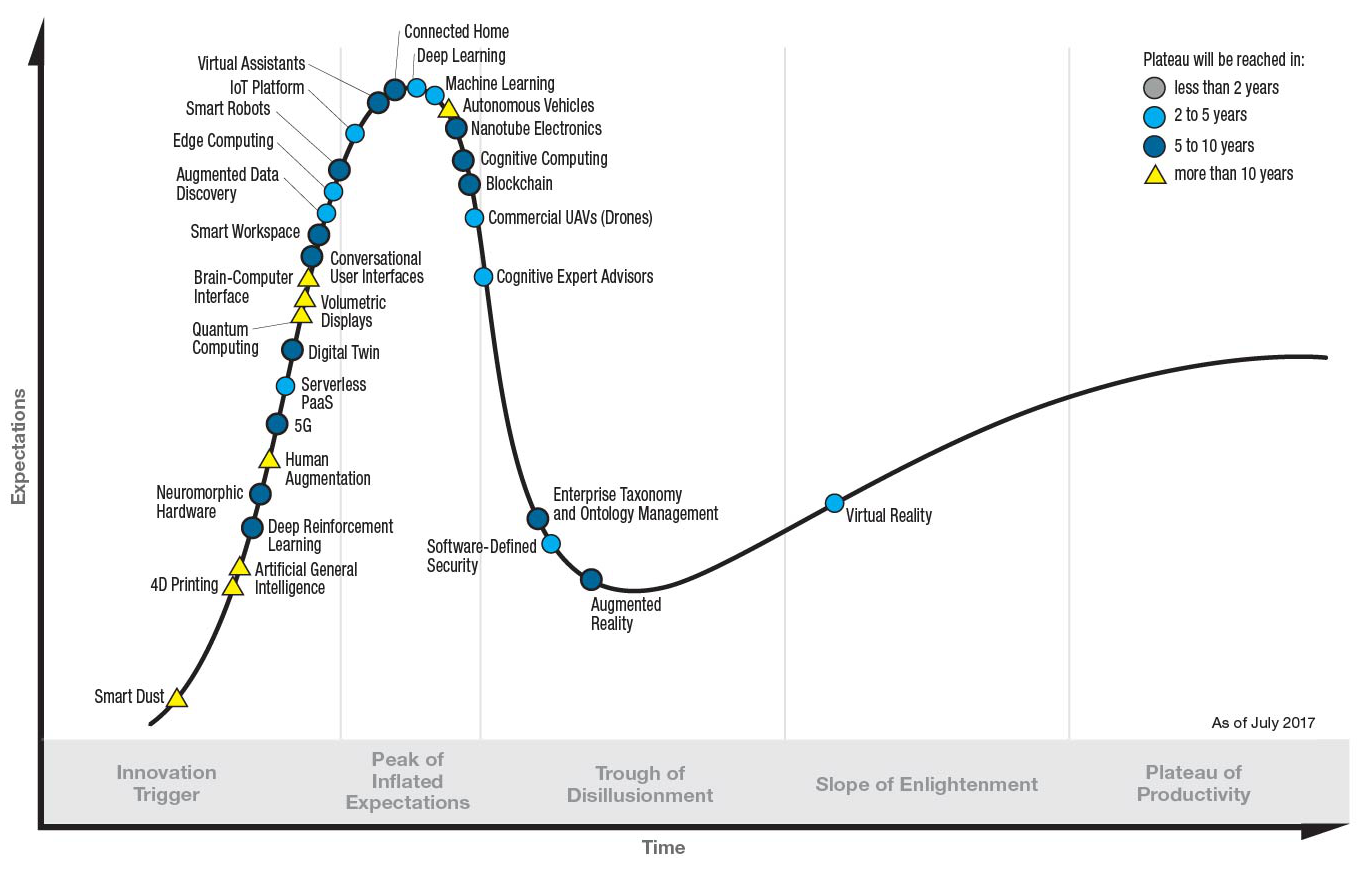
\includegraphics[width=0.65\linewidth]{pictures/Gartner-Hype-Cycle-2017}
	\caption[Gartner Hype Cycle 2017]{Emerging Technologies Hype Cycle 2017\cite{Gartner2017}}
	\label{fig:gartner-hype-cycle-2017}
\end{figure}

Noch ist die Blockchain jedoch kein Alltag, bemessen am jährlich erscheinenden Hype Cycle des Marktforschungsinstituts Gartner, Inc. $( Abb.~ \ref{fig:gartner-hype-cycle-2017} )$ hat die Technologie noch fünf bis zehn Jahre Entwicklungszeit vor sich. Erst dann wird sie nach aktueller Einschätzung im produktiven Einsatz sein.\\

Bereits heute zeigen sich signifikante Unterschiede zwischen den unzähligen Blockchains die in Pilotprojekten realisiert wurden. So gibt es Anwendungen der Blockchain um beispielsweise den Kilometerstand eines Fahrzeugs täglich \glqq in die Blockchain\grqq~ zu schreiben. Die inhärenten Eigenschaften der Blockchain ermöglichen es sehr einfach festzustellen, ob ein Kilometerstand nachträglich durch Fremdeinwirkung manipuliert wurde. Ebenfalls ist keine zentrale \glqq Clearing Stelle\grqq{} bzw. Supervisor mehr nötig, um für die Echtheit des hinterlegten Wertes zu garantieren. \cite{carVertical}\\

Bitcoin war die erste Generation von Blockchain. Die Bitcoin Blockchain ist in der Lage Einheiten der Bitcoin Währung zwischen zwei Parteien zu versenden ohne das eine Bank oder eine Clearingstelle diese Transaktion validieren muss. \cite[vgl.]{Nakamoto2009} Ethereum war die zweite Generation einer Blockchain. Im Vergleich zur Bitcoin Blockchain lassen sich mit dem Ethereum Netzwerk auch sog. \ac{sc} erstellen und ausführen.\cite[vgl.]{Buterin2014} Skalierbarkeit und Interoperabilität spielen in dieser Generation eine der entscheidenden Rollen. \cite[vgl.]{Cardano} Blockchain Anwendungen im Enterprise Bereich exisiteren maximal auf dem Reißbrett.\\

Die Kernidee hinter der Blockchain-Technologie ist es einen Intermediär zu substituieren, der nur eingesetzt wurde um eine neutrale Vertrauensbildung zu ermöglichen. \ac{dlt} verfolgt dabei den Ansatz die Vertrauensbildung, den Ablauf von Transaktionen und deren sichere Festschreibung mit mathematischen und kryptographischen Methoden zu realisieren. Im Kontrast zum konventionellen Intermediär, welcher durch eine dritte Person oder Institution wie z.B. eine Bank oder einen Notar repräsentiert wird.\\

Für das Problem der Einigkeit über den Zustand eines Werts innerhalb der Blockchain sind zwei generelle Verfahren etabliert. Die \ac{pow} und \ac{pos} genannten Algorithmen nutzen unterschiedliche Ansätze um Konsens innerhalb eines Netzwerks zu bilden und so Vertrauen herzustellen. Beide Verfahren haben ihre Vor- und Nachteile.\\

Prozesse die einen transaktionalen Charakter besitzen und oft auch ein oder mehrere Vermittlerstellen zwischengeschaltet haben würden sich Ideal für den Einsatz von Blockchain Technologie eignen. Fehlende Standards und generelle Unsicherheit verhindern allerdings den flächendeckenden Einsatz der Technologie.\\

Abbildung \ref{fig:statista-huerden-blockchain-2016} zeigt die Ergebnisse einer Umfrage des Fachmagazins Cofinpro zum Thema \glqq Wo sehen Sie Hürden für die Blockchain-Technologie?\grqq~. So scheinen die mit Abstand größten Einstiegsbarrieren fehlende Standards und rechtliche Regelungen zu sein.

\begin{figure}[h!]
	\centering
	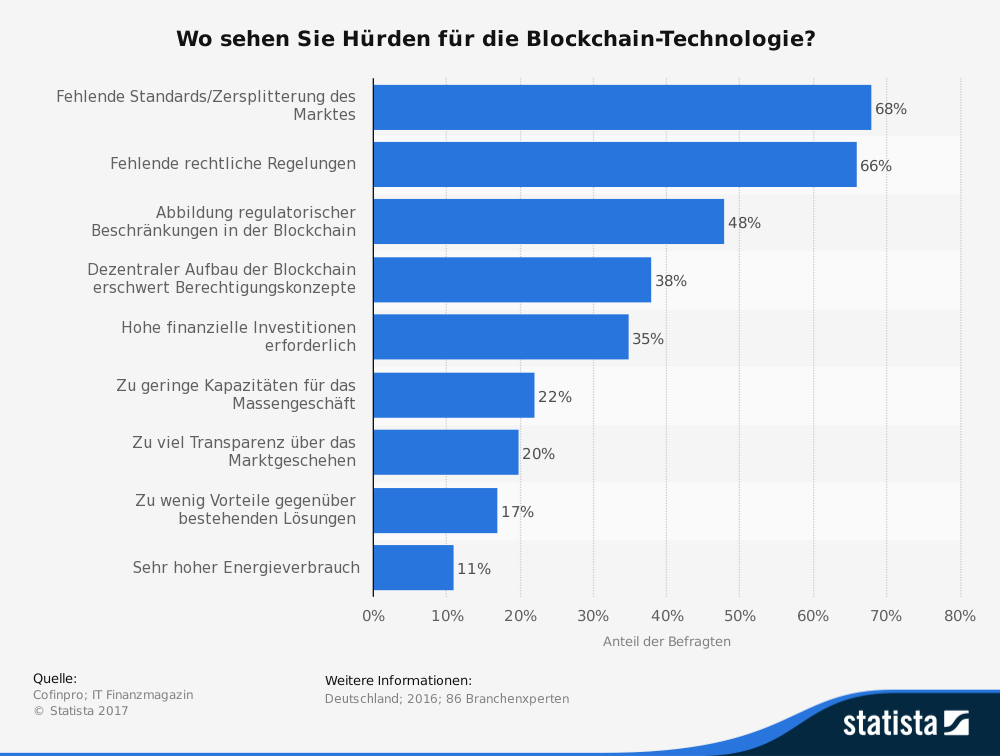
\includegraphics[width=0.7\linewidth]{pictures/Statista-Huerden-Blockchain-2016}
	\caption[Statista Blockchain Umfrage]{Cofinpro - Wo sehen Sie Hürden für die Blockchain Technologie? \cite{Cofinpro}}
	\label{fig:statista-huerden-blockchain-2016}
\end{figure}


\newpage
